\documentclass[UTF8,a4paper,10pt]{ctexart}
\usepackage[left=2.00cm, right=2.00cm, top=3.50cm, bottom=3.50cm]{geometry} %页边距
\CTEXsetup[format={\Large\bfseries}]{section} %设置章标题居左
 
 
%%%%%%%%%%%%%%%%%%%%%%%
% -- text font --
% compile using Xelatex
%%%%%%%%%%%%%%%%%%%%%%%
% -- 中文字体 --
%\setmainfont{Microsoft YaHei}  % 微软雅黑
%\setmainfont{YouYuan}  % 幼圆    
%\setmainfont{NSimSun}  % 新宋体
%\setmainfont{KaiTi}    % 楷体
%\setmainfont{SimSun}   % 宋体
%\setmainfont{SimHei}   % 黑体
% -- 英文字体 --
%\usepackage{times}
%\usepackage{mathpazo}
%\usepackage{fourier}
%\usepackage{charter}
\usepackage{helvet}
\usepackage{amsmath, amsfonts, amssymb} % math equations, symbols
\usepackage[english]{babel}
\usepackage{color}      % color content
\usepackage{graphicx}   % import figures
\usepackage{subfig}
\usepackage{url}        % hyperlinks
\usepackage{bm}         % bold type for equations
\usepackage{multirow}
\usepackage{booktabs}
\usepackage{epstopdf}
\usepackage{epsfig}
\usepackage{algorithm}
\usepackage{algorithmic} 
\usepackage{listings} 
\usepackage{xcolor}
\lstset{
    language=matlab,  %代码语言使用的是matlab
    frame=shadowbox, %把代码用带有阴影的框圈起来
    rulesepcolor=\color{red!20!green!20!blue!20},%代码块边框为淡青色
    keywordstyle=\color{blue!90}\bfseries, %代码关键字的颜色为蓝色,粗体
    commentstyle=\color{red!10!green!70}\textit,    % 设置代码注释的颜色
    showstringspaces=false,%不显示代码字符串中间的空格标记
    numbers=left, % 显示行号
    numberstyle=\tiny,    % 行号字体
    stringstyle=\ttfamily, % 代码字符串的特殊格式
    breaklines=true, %对过长的代码自动换行
    extendedchars=false,  %解决代码跨页时,章节标题,页眉等汉字不显示的问题
%   escapebegin=\begin{CJK*},escapeend=\end{CJK*},      
% 代码中出现中文必须加上,否则报错
    texcl=true}
\renewcommand{\algorithmicrequire}{ \textbf{Input:}}     % use Input in the format of Algorithm  
\renewcommand{\algorithmicensure}{ \textbf{Initialize:}} % use Initialize in the format of Algorithm  
\renewcommand{\algorithmicreturn}{ \textbf{Output:}}     % use Output in the format of Algorithm   

% -------------------------允许算法跨页-------------
\makeatletter
\newenvironment{breakablealgorithm}
    {% \begin{breakablealgorithm}
    \begin{center}
        \refstepcounter{algorithm}% New algorithm
        \hrule height.8pt depth0pt \kern2pt% \@fs@pre for \@fs@ruled
        \renewcommand{\caption}[2][\relax]{% Make a new \caption
            {\raggedright\textbf{\ALG@name~\thealgorithm} ##2\par}%
                \ifx\relax##1\relax % #1 is \relax
                    \addcontentsline{loa}{algorithm}{\protect\numberline{\thealgorithm}##2}%
                \else % #1 is not \relax
                    \addcontentsline{loa}{algorithm}{\protect\numberline{\thealgorithm}##1}%
                \fi
            \kern2pt\hrule\kern2pt
        }
  }{% \end{breakablealgorithm}
            \kern2pt\hrule\relax% \@fs@post for \@fs@ruled
        \end{center}
  }
\makeatother
 
\usepackage{fancyhdr} %设置页眉、页脚
%\pagestyle{fancy}
\lhead{}
\chead{}
%\rhead{\includegraphics[width=1.2cm]{fig/ZJU_BLUE.eps}}
\lfoot{}
\cfoot{}
\rfoot{}
%\pagestyle{empty} %删除所有页码
 
%%%%%%%%%%%%%%%%%%%%%%%
%  设置水印
%%%%%%%%%%%%%%%%%%%%%%%
%\usepackage{draftwatermark}         % 所有页加水印
%\usepackage[firstpage]{draftwatermark} % 只有第一页加水印
% \SetWatermarkText{Water-Mark}           % 设置水印内容
% \SetWatermarkText{\includegraphics{fig/ZJDX-WaterMark.eps}}         % 设置水印logo
% \SetWatermarkLightness{0.9}             % 设置水印透明度 0-1
% \SetWatermarkScale{1}                   % 设置水印大小 0-1    
 
\usepackage{hyperref} %bookmarks
\hypersetup{colorlinks, bookmarks, unicode} %unicode
 

\title{\textbf{数值代数第3章上机实验报告}}
\author{ 211840196 张博阳 }
\date{}


\begin{document}
    \maketitle
 
    \section*{摘要}
        \par
        本实验报告基于第3章所学最小二乘问题的数值理论知识,对上机实验题给出了相应的程序实现与执行情况,主要聚焦于不同直交化方法和正规化与直交化求解最小二乘问题的性能比较,在代码实现上尤其注重低秩修正设计对运算速度的提升,并基于程序执行情况对不同方法的性能进行了评价与理论对照。

    \section{前言}
        \par
        对于矛盾方程组($m>n$)的情形,一般方程组没有通常意义下的解,此时通常考虑寻求其最小二乘解,常用的方法是正规化求解方法,即法方程组法和直交化求解方法。本次数值实验的前两个问题对不同的矩阵直交化方法和最小二乘解求解方法进行了数值观察,第三个实验观察奇异值分解对不同图像在图像恢复上的不同效果,不同图像主要关注图像内元素是否存在清晰光滑的边缘。
        
    \section{数学原理和程序设计流程}
        \par
        直交化方法的主要手段为经典Gram-Schmidt直交化方法(CGS)、改进Gram-Schmidt直交化方法(MGS)的直接直交算法及利用Householder或Givens阵消零的直交阵算法。根据理论分析结果,在实验观察的几种算法中:Householder方法具有更好的列直交性和更低的计算复杂度;MGS方法其次,仅在列直交性表现上弱于Householder方法;Givens方法具有较好的列直交性表现,但计算复杂度显著提升;CGS方法在复杂度上与MGS方法基本相同,但舍入误差影响更大,导致列直交性表现和数值误差表现不如MGS方法。
        \par
        各方法的列直交性有如下结果
        $$
        \left\|Q_{MGS}^{\mathrm{T}}Q_{MGS}-I\right\|_2\le c_{mn}\vartheta\kappa_2(A)+\mathrm{O}((\vartheta\kappa_2(A))^2)
        $$
        $$
        \left\|H_{num}^{\mathrm{T}}H_{num}-I\right\|\le c\vartheta,H_{num}=\prod_{k=1}^{n}H_k
        $$
        $$
        \left\|G_{num}^{\mathrm{T}}G_{num}-I\right\|\le c\vartheta
        $$
        \par
        各方法的乘除次数有如下结果
        $$
        N_{GS}=\mathrm{O}(mn^2)
        $$
        $$
        N_{Householder}=\mathrm{O}\left(mn^2-\frac{n^3}{3}\right)
        $$
        $$
        N_{Givens}=\mathrm{O}\left(2mn^2-\frac{2n^3}{3}\right)
        $$
        其中对于稠密矩阵,Givens方法含有至少$\mathrm{O}(n)$量级次数的开根号运算。
        \par
        正规化求解方法的主要手段是构造对应问题的法方程组直接求解或者等价的Karush-Kuhm-Tucker扩展法方程组迭代求解,在解决$m>>n$的问题时,问题的规模将得到较大程度上的下降,而当$m$和$n$差距不大时,根据$\kappa(A^\mathrm{T}A)= \kappa(A)^2$,问题的病态程度急剧增大,将影响法方程组的求解。问题6.3.2针对一个$n\times(n-1)$阶矩阵的最小二乘问题,法方程组的规模达到$n^2$量级且问题病态程度增大,数值效果应当不如直交化手段求解最小二乘问题。
        \par
        在程序设计上,重点考虑了Householder矩阵
        $$
        H=I-b^{-1}uu^{\mathrm{T}}
        $$
        和Givens矩阵
        $$
        G(i,j;\theta)=
        \begin{bmatrix}
            I_{i-1} & \ & \ & \ & \ \\
            \ & \cos\theta & \ & \sin\theta & \ \\
            \ & \ & I_{j-i-1} & \ & \ \\
            \ & -\sin\theta & \ & \cos\theta & \ \\
            \ & \ & \ & \ & I_{n-j}
        \end{bmatrix}
        $$
        作为单位阵的低秩修正带来的计算优势。对于任意$A=\left[\alpha_1\ \alpha_2\cdots\alpha_n\right]\in M_n(\mathbb{R})$,
        $$
        \begin{aligned}
            HA&=\left(I-b^{-1}uu^{\mathrm{T}}\right)\left[\alpha_1\ \alpha_2\ \cdots\ \alpha_n\right] \\
            &=\left[\alpha_1-b^{-1}\left(u^{\mathrm{T}}\alpha_1\right)u\ \alpha_2-b^{-1}\left(u^{\mathrm{T}}\alpha_2\right)u \ \cdots \ \alpha_n-b^{-1}\left(u^{\mathrm{T}}\alpha_n\right)u\right]
        \end{aligned}
        $$
        计算复杂度由$\mathrm{O}(n^3)$下降至$\mathrm{O}(n^2)$。特别地,若$H$是对某一列的消零Householder阵,可采用该列只算对角元,其他元素直接置0的方
        式进一步降低计算量。
        \par
        对于任意$\alpha\in\mathbb{R}^n$,
        $$
        G(i,j;\theta)\alpha=
        \begin{bmatrix}
            I_{i-1} & \ & \ & \ & \ \\
            \ & \cos\theta & \ & \sin\theta & \ \\
            \ & \ & I_{j-i-1} & \ & \ \\
            \ & -\sin\theta & \ & \cos\theta & \ \\
            \ & \ & \ & \ & I_{n-j}
        \end{bmatrix}
        \begin{bmatrix}
            a(1:i-1) \\
            a_i \\
            a(i+1:j-1) \\
            a_j \\
            a_(j+1:n)
        \end{bmatrix}
        =
        \begin{bmatrix}
            a(1:i-1) \\
            a_i\cos\theta+a_j\sin\theta \\
            a(i+1:j-1) \\
            -a_i\sin\theta+a_j\cos\theta \\
            a_(j+1:n)
        \end{bmatrix}
        $$
        计算复杂度由$\mathrm{O}(n^2)$下降至常数量级,特别地,若引入置0策略,复杂度可进一步降低。这进一步体现了Givens处理稀疏矩阵的优势,但本次实验均为稠密矩阵,Givens方法的计算量主体来自每次消元Givens阵参数的计算。
\section{实验结果和数据讨论}
    \subsection{练习6.3.1}
        \par
        练习6.3.1的实验结果如Figure 1-3所示。
        \par
        在列直交性表现上,四种算法的表现与理论分析相吻合,同时基于直交矩阵的直交化方法展现出稳定的列直交性,而直接直交化方法存在较大的波动。
        \par
        在CPU运行时间上,Householder和Givens的关系与理论分析相合,但Householder运行时间长于直接直交化方法。通过代码性能探查,以随机生成的1000阶矩阵作测试,Householder方法共用12.340秒,其中主要部分为计算$Q$(7.937秒)和计算每一步消零后的$A$(4.246秒),而MGS方法共用2.110秒,其中主要部分为计算$R$(1.261秒)和计算每一步直交化后的$A$(0.791秒),考虑可能是内存开辟与管理机制作用下的结果。代码探查报告见附件\texttt{mgs\_report.pdf}和\texttt{household\_report.pdf}。
        \par
        在后验误差上,直接直交化算法的表现好于基于直交阵的直交化算法,数量级分别在$10^{-14}$和$10^{-13}$左右,均给出了满意的结果。
        \par
        在直接直交化算法和基于直交阵的直交化算法内部比较,MGS方法在各个指标上均优于CGS算法。由于本实验题采用稠密矩阵,因此Householder方法在各个指标上均优于Givens方法。
    \subsection{练习6.3.2}
        \par
        练习6.3.2的实验结果如Figure 4-5所示。
        \par
        对于线性方程组的求解,本题采用第2章所学的CG算法求解,用户指标设定为$10^{-12}$。一方面,由于矩阵的行列差距较小,从而法方程组的规模以平方关系上升,条件数亦平方上升,故正规化求解方法的数值表现均较差,CPU运行时间和数值误差均随$n$的增大而快速上升。另一方面,根据代码探查结果,CG算法的执行时间占总算法时间的99.5\%以上,而用户指标设定是基于其他算法反馈的数值结果设定的。总而言之,正规化求解方法无法在两个指标上均与直交化求解方法抗衡。
        \par
        三种直交化求解方法数值表现相当,Givens方法表现最差,MGS方法在CPU运行时间上占优,而Householder方法在数值误差表现上占优。
    \subsection{练习6.3.3}
        \par
        练习6.3.2的实验结果如Figure 6-7所示。
        \par
        实验选用了两张照片:一张为英国球星David Beckham的图片,轮廓较为清晰;另一张为峨眉山金顶云海的景观图,不具有清晰的轮廓。两张照片均为768$\times$1024规格。分别取$k=5,10,50$观察效果。当$k=50$时两组图片均被大致恢复,但云海组图片丢失了大量细节,球员组除手臂白色部分,其他细节均大致恢复。由此可见,图片自身轮廓是否具有清晰特征影响奇异值分解对于图像的压缩和恢复效果。

\section{小结}
    \par
    通过上述实验题,直接直交化方法和基于直交矩阵的直交化方法在数值表现上各有长处。对于求解线性最小二乘问题,由于问题自身性质的限制,正规化求解方法被限制,没有给出好的数值结果,但直交化方法均给出了令人满意的结果。不同的方法均有其适用的问题,需要根据具体问题选取合适的求解方法。

    \begin{figure*}[ht]
        \centering
        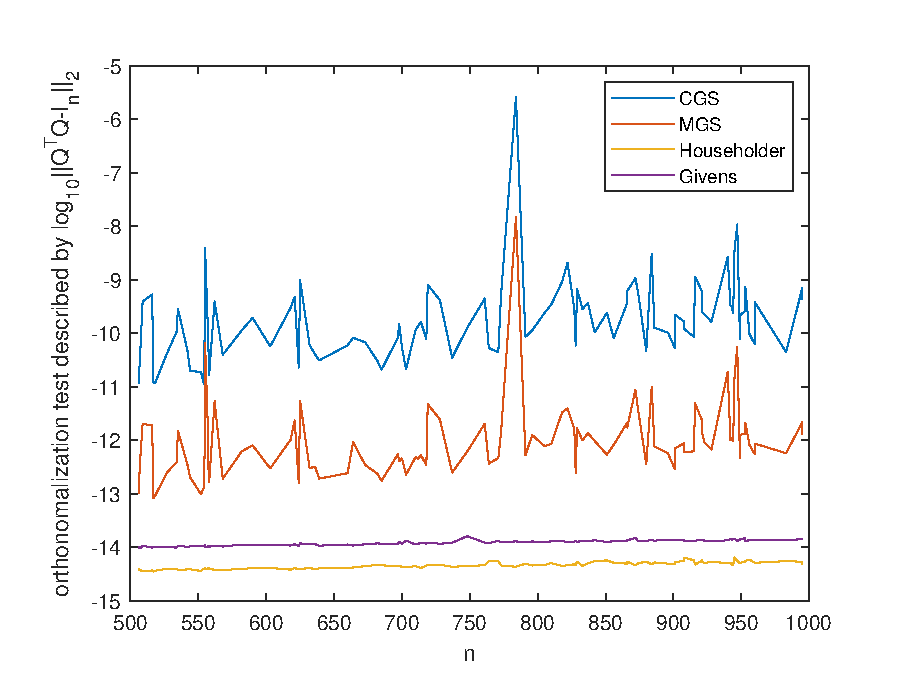
\includegraphics[width=14cm,height=10cm]{1_orthonomalization.eps}
        \caption{Orthonomalization test}
    \end{figure*}
    \begin{figure*}[ht]
        \centering
        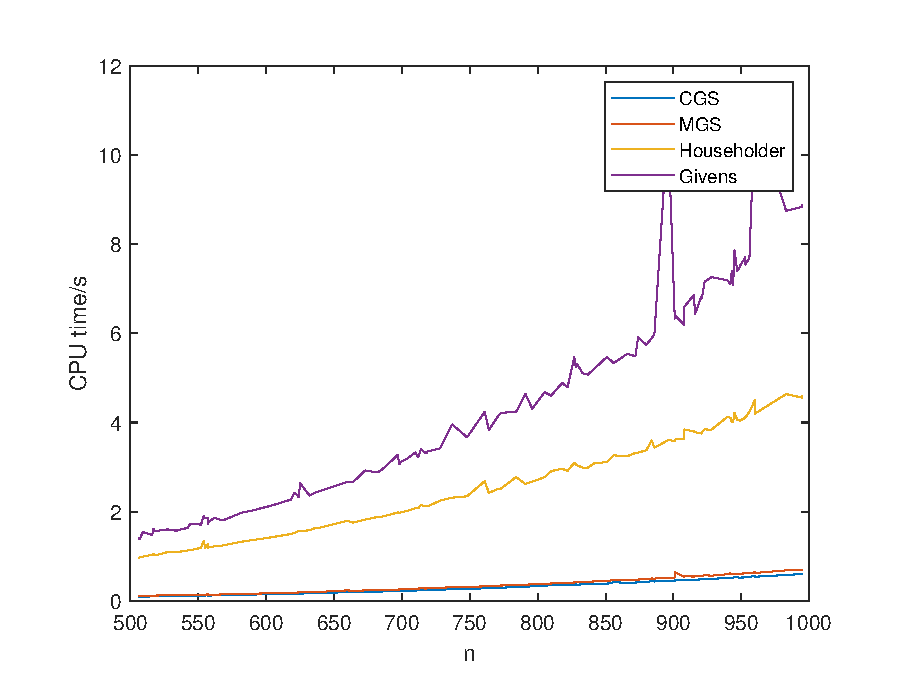
\includegraphics[width=14cm,height=10cm]{1_CPU.eps}
        \caption{CPU running time}
    \end{figure*}
    \begin{figure*}[ht]
        \centering
        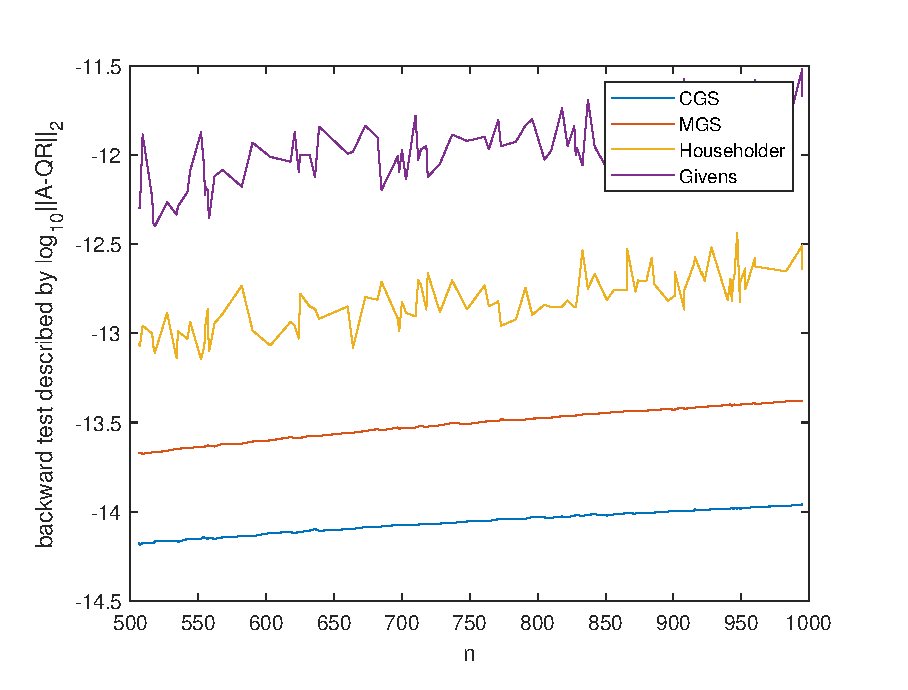
\includegraphics[width=14cm,height=10cm]{1_backward.eps}
        \caption{Backward error test}
    \end{figure*}

\begin{figure*}[ht]
    \centering
    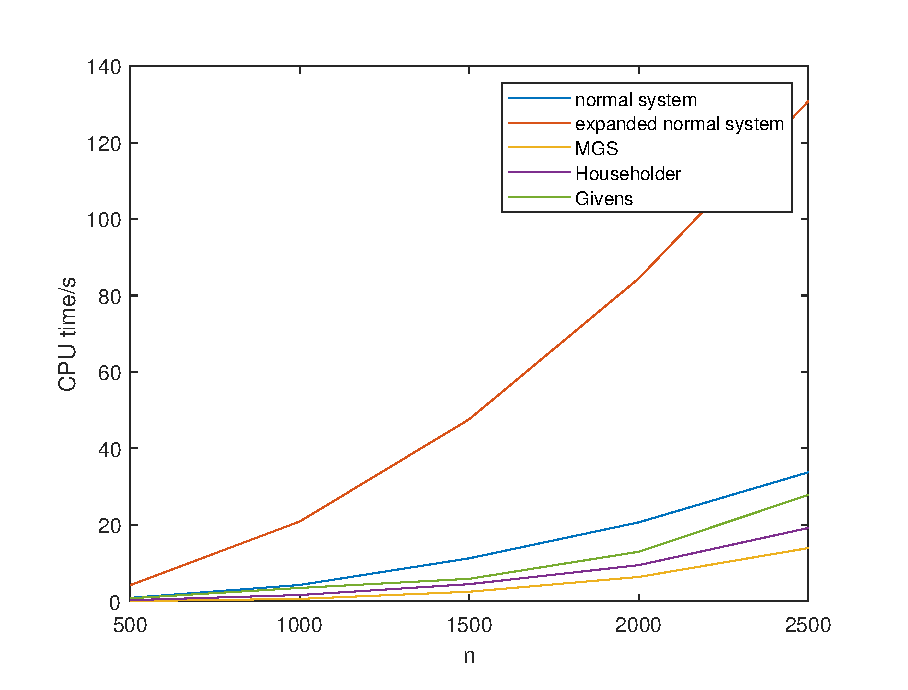
\includegraphics[width=14cm,height=10cm]{2_CPU.eps}
    \caption{The numerical error using the remaining rule and 1-norm}
\end{figure*}
\begin{figure*}[ht]
    \centering
    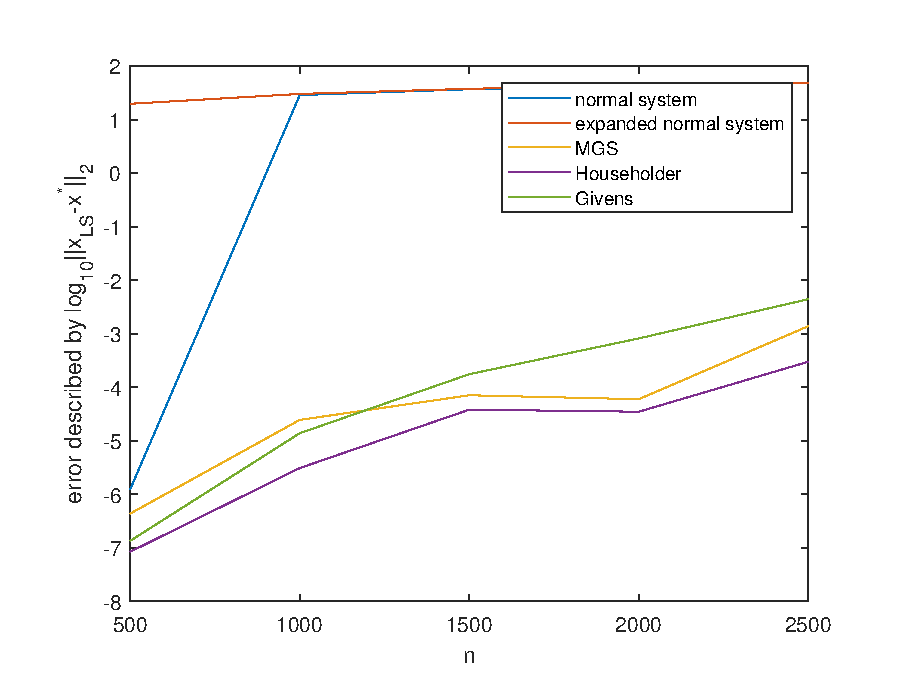
\includegraphics[width=14cm,height=10cm]{2_error.eps}
    \caption{The numerical error using the remaining rule and 1-norm}
\end{figure*}

\begin{figure}[htbp]
    \centering
    \subfloat[原图]
    {\includegraphics[width=0.4\textwidth]{3\_1.eps}}
    [b]     % 重点就在这,优先横向排列,自动换行
    \subfloat[$k=5$]
    {\includegraphics[width=0.4\textwidth]{3\_1\_1.eps}}
    [b]
    \subfloat[$k=10$]
    {\includegraphics[width=0.4\textwidth]{3\_1\_2.eps}}
    [b]
    \subfloat[$k=50$]
    {\includegraphics[width=0.4\textwidth]{3\_1\_3.eps}}
    [b]
    \caption{David Beckham图片压缩与恢复}
  \end{figure}
  \begin{figure}[htbp]
    \centering
    \subfloat[原图]
    {\includegraphics[width=0.4\textwidth]{3\_2.eps}}
    [b]     % 重点就在这,优先横向排列,自动换行
    \subfloat[$k=5$]
    {\includegraphics[width=0.4\textwidth]{3\_2\_1.eps}}
    [b]
    \subfloat[$k=10$]
    {\includegraphics[width=0.4\textwidth]{3\_2\_2.eps}}
    [b]
    \subfloat[$k=50$]
    {\includegraphics[width=0.4\textwidth]{3\_2\_3.eps}}
    [b]
    \caption{峨眉山金顶云海图片压缩与恢复}
  \end{figure}

    
\section*{参考文献}
[1]林成森. 数值计算方法(下册)[M]. 北京: 科学出版社, 2005.
\end{document}

